% mainfile: ../../../main.tex
\chapter{Additional measurements}\label{ch:app:exp:observations}
In this appendix, I give additional information on simulation parameters and show further measurements.

\section{Self-consistent Poisson-Schrödinger simulation of the membrane band structure}\label{sec:app:exp:observations:ps}
\begin{margintable}
    \centering
    \footnotesize
    \caption{
        Heterostructure parameters used in \thethesis.
        The doping density $N_{\mr{d}}$ is nominal, whereas the charge carrier density in the \gls{qw}, $n$, is computed using the nominal doping values with parameters given in \cref{tab:app:exp:samples:ps}.
    }
    \label{tab:app:exp:samples}
    \begin{tabularx}{\marginparwidth}{@{} l @{} S[table-alignment=right, table-format=1.1e1] S[table-alignment=right, table-format=1.2e2] @{}}
        \toprule
        \textsc{Wafer}          & {$N_{\mr{d}}$ (\unit{\per\cubic\centi\meter})} & {$n$ (\unit{\per\square\centi\meter})} \\
        \midrule
        \textsc{M1\_05\_49}     & 6.5e17                                         & 1.95e11 \\
        \textsc{15460 (Honey)}  & 1.8e18                                         & 4.26e11 \\
        \textsc{15271 (Fig)}    & 8.0e17                                         & 3.91e11 \\
        \bottomrule
    \end{tabularx}
\end{margintable}
\begin{margintable}
    \centering
    \footnotesize
    \begin{threeparttable}
        \caption{
            Simulation parameters used to compute the charge carrier density $n$ in \cref{tab:app:exp:samples}.
        }
        \label{tab:app:exp:samples:ps}
        \begin{tabularx}{\marginparwidth}{c S l}
            \toprule
            \textsc{Parameter}              & {\textsc{Value}}  & \textsc{Unit} \\
            \midrule
            $E_{\mr{DX}}$\tnote{a}          & -71.5             & \unit{meV} \\
            $\Delta E_{\mr{c}}$\tnote{b}    & 240               & \unit{meV} \\
            $m_{\mr{c}}$                    & 0.067             & $m_e$ \\
            $\Delta z$                      & 0.5               & \unit{nm} \\
            $T$                             & 10                & \unit{mK} \\
            $V_{\mr{FP}}$\tnote{c}          & 0.76              & \unit{V} \\
            \bottomrule
        \end{tabularx}
        \begin{tablenotes}
            \scriptsize
            \item[a] Energy of the DX-center below the Fermi level.
            \item[b] Conduction band offset at the \ch{GaAs/AlGaAs} interface.
            \item[c] Fermi level pinning voltage.
        \end{tablenotes}
    \end{threeparttable}
\end{margintable}

The samples studied in \cref{ch:exp:observations} were all grown using \gls{mbe} and had similar nominal designs.
To compare the design charge carrier density with the measurements obtained from \gls{pl} of the Fermi edge, I simulated the band structure using a self-consistent Poisson-Schrödinger solver~\cite{PoissonSchroedinger}.
\Cref{tab:app:exp:samples} shows the nominal doping concentration $N_{\mr{d}}$ as well as the charge carrier density in the \gls{qw}, $n$, obtained from a simulation using the parameters given in \cref{tab:app:exp:samples:ps}.

\section{Additional data}\label{sec:app:exp:observations:meas}
\subsection{Combined plot of \texorpdfstring{\acrshort{pl}}{PL} and \texorpdfstring{\acrshort{ple}}{PLE} data}\label{subsec:app:exp:observations:meas:pl_ple}
\begin{figure}
    \centering
    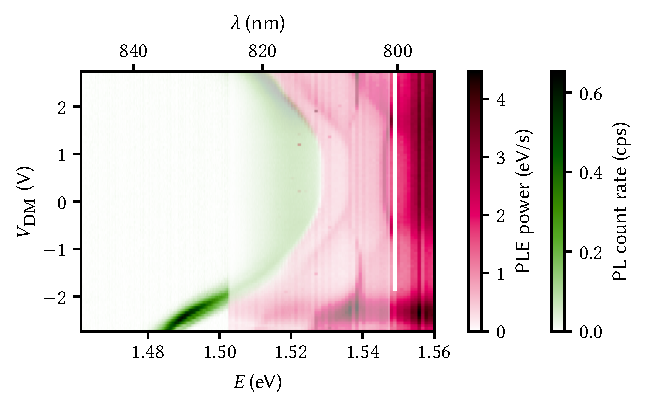
\includegraphics{img/pdf/experiment/doped_M1_05_49-2_ple_single}
    \caption[
        \sampleid{Doped M1_05_49-2}
        \thevoltage{-1.3}{CM}
        \thepower{1}{\micro}
        \protect\newline
        \imgsource{img/py/experiment/ple.py}
    ]{
        Combined plot of the \gls{pl} with excitation at \qty{795}{\nano\meter} (green) and \gls{ple} (magenta).
        The data overlap in the range of \qtyrange{801}{825}{\nano\meter}, where they are plotted with \qty{50}{\percent} transparency.
        The onset of the absorption edge in \gls{ple} coincides with the high-energy shoulder of the \gls{pl} emission.
    }
    \label{fig:app:exp:pl:doped_M1_05_49-2_ple}
\end{figure}

In \cref{sec:exp:observations:ple}, I showed \gls{ple} measurements of a large exciton trap.
When integrating the \gls{pl} spectrum over the detection energy, the data showed several distinct features including an onset of the absorption that depends on the electric field applied by the difference-mode voltage \VDM.
\Cref{fig:app:exp:pl:doped_M1_05_49-2_ple} shows the same data as panels (a) and (b) of \cref{fig:exp:pl:doped_M1_05_49-2_ple}, but drawn in the same plot.
It is clear that the onset of absorption occurs just as the \gls{pl} emission drops off, indicating a small Stokes shift.

\subsection{\texorpdfstring{\acrshort{2deg}}{2DEG} \texorpdfstring{\acrshort{pl}}{PL} as function of power}\label{subsec:app:exp:observations:meas:2deg}
\begin{figure}
    \centering
    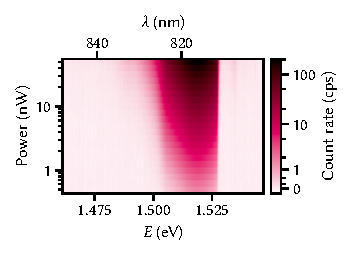
\includegraphics{img/pdf/experiment/2deg_pl_power_dependence}
    \caption[
        \sampleid{Doped M1_05_49-2}
        \thewavelength{795}
        \protect\newline
        \imgsource{img/py/experiment/pl.py}
    ]{
        \Gls{2deg} \gls{pl} of an unbiased \gls{qw} as function of excitation power.
        The Fermi edge at \qty{1.5275}{\electronvolt} does not broaden over two orders of magnitude as the line cuts in the upper panels also show.
    }
    \label{fig:app:exp:observations:2deg_pl_power_dependence}
\end{figure}

In \cref{sec:exp:observations:pl}, it was determined that the electrons recombining from the Fermi edge of the \gls{2deg} were much hotter at $\sim\qty{1}{\kelvin}$ than the cryostat temperature at $\sim\qty{10}{\milli\kelvin}$.
The fit to the trion-exciton lineshape in \cref{sec:exp:observations:ple} yielded similar results.
\Cref{fig:app:exp:observations:2deg_pl_power_dependence} demonstrates that this is not a local heating of the lattice due to excess laser power.
Shown is the \gls{2deg} \gls{pl} as function of excitation power from \qtyrange{5}{500}{\nano\watt}, with the upper panel showing line cuts at highest and lowest power.
There is no discernible broadening in the Fermi edge on the high-energy side of the spectrum.
